\section{Auswertung}
\label{sec:Auswertung}

\noindent Bei der Versuchsvorbereitung und wird der Rezipient zuerst mit der Drehschieberpumpe evakuiert. Dabei wird der Druck $p_\text{E}$ ermittelt, welcher der kleinst erreichbare Druck 
der Vakuumpumpe ist. Der Wert beträgt $p_\text{E} = \SI{3.85(115)e-3}{\milli\bar}$. Anschließend wird die Turbopumpe eingeschalten und auch von ihr der Enddruck bestimmt, welcher hier 
$p_\text{E} = \SI{10.9 \pm 3.27}{\nano\bar}$ beträgt. 

\subsection{Turbopumpe}

  \noindent Zuerst wurden die Messungen mit der Turbomolekularpumpe durchgeführt, mit der Leckratenmessung wurde begonnen. Das Volumen des benutzten Rezipienten beträgt $V = \SI{33 \pm 3.3}{L}$. 
  
  \subsubsection{Leckratenmessung}

    \noindent Es wurde, wie in der \autoref{sec:Durchführung} beschrieben ein Gleichgewichtsdruck von $p_\text{G} = \SI{50}{\nano\bar}, \, \SI{70}{\nano\bar}, \,  \SI{100}{\nano\bar},\, \SI{200}{\nano\bar}$ eingestellt 
    und bei $t = \SI{0}{\second}$ die Pumpe abgeschiebert und in Schritten von $\increment t = \SI{10}{\second}$ der Druck an dem Messgerät M2 abgelesen. Dies wurde 3 mal für jeden 
    Gleichgewichtsdruck gemacht. Anschließend wurden die Drücke der Messung pro Zeit gemittelt. Die Messwerte der einzelnen Messungen und der gemittelte Druck sind für $p_\text{G} = \SI{100}{\nano\bar}$ in der \autoref{tab:turbo_leck_1}, für 
    $\SI{200}{\nano\bar}$ in der \autoref{tab:turbo_leck_2}, für $p_\text{G} = \SI{50}{\nano\bar}$ in der \autoref{tab:turbo_leck_5} und schließlich für $\SI{70}{\nano\bar}$ in der \autoref{tab:turbo_leck_7} zu finden. 

    \begin{figure}[h]
      \begin{subfigure}{0.48\textwidth}
        \centering
        \includegraphics[width=\textwidth]{build/leck_turbo_50nbar.pdf}
        \caption{Gleichgewichtsdruck $p_\text{G} = \SI{50}{\nano\bar}$.}
        \label{fig:turbo_leck_50}
      \end{subfigure}
      \hfill
      \begin{subfigure}{0.48\textwidth}
        \centering
        \includegraphics[width=\textwidth]{build/leck_turbo_70nbar.pdf}
        \caption{Gleichgewichtsdruck $p_\text{G} = \SI{70}{\nano\bar}$.}
        \label{fig:turbo_leck_70}
      \end{subfigure}
      \hfill
      \begin{subfigure}{0.48\textwidth}
        \centering
        \includegraphics[width=\textwidth]{build/leck_turbo_100nbar.pdf}
        \caption{Gleichgewichtsdruck $p_\text{G} = \SI{100}{\nano\bar}$.}
        \label{fig:turbo_leck_100}
      \end{subfigure}
      \hfill
      \begin{subfigure}{0.48\textwidth}
        \centering
        \includegraphics[width=\textwidth]{build/leck_turbo_200nbar.pdf}
        \caption{}Gleichgewichtsdruck $p_\text{G} = \SI{200}{\nano\bar}$.
        \label{fig:turbo_leck_200}
      \end{subfigure}
      \caption{Die gemittelten Drücke der Messungen  der Drehschieberpumpe zu den verschiedenen Gleichgewichtsdrücken mit der jeweiligen linearen Ausgleichsrechnung.}
      \label{fig:turbo_leck}
    \end{figure}

    \noindent Die gemittelten Drücke werden gegen die Zeit in einem $t-p$ Diagramm dargestellt. Diese sind für die verschiedenen Gleichgewichtsdrücke in der \autoref{fig:turbo_leck} dargestellt. 
    Es werden keine Messdaten exkludiert.  
    Zusätzlich ist jeweils ein Fit der Form $p(t) = m \cdot t + n $ eingezeichnet. Dieser wird mithilfe von python \cite{scipy} gemacht. Die Fitparameter ergeben sich zu den folgenden Werten. 
    \begin{align*}
      \text{Für} \quad  p_\text{G} &= \SI{50}{\nano\bar} & \text{Für} \quad  p_\text{G} &= \SI{70}{\nano\bar}\\
      m &= \SI{11.22 \pm 0.48}{\nano\bar\per\second} & m &= \SI{19.28 \pm 0.86}{\nano\bar\per\second} \\
      n &= \SI{-7.86 \pm 33.73}{\nano\bar} & n &= \SI{-91.84 \pm 61.03}{\nano\bar} \\
      \\
      \text{Für} \quad  p_\text{G} &= \SI{100}{\nano\bar} & \text{Für} \quad  p_\text{G} &= \SI{200}{\nano\bar}\\
      m &= \SI{53.94(207)}{\nano\bar\per\second} & m &= \SI{191.95 \pm 2.31}{\nano\bar\per\second} \\
      n &= \SI{-424.08 (14611)}{\nano\bar} & n &= \SI{-342.78 \pm 163.26}{\nano\bar} 
    \end{align*} 

    \noindent Durch Vergleich mit der Gleichung \eqref{eq:saug_leck_theorie} folgt, dass das Saugvermögen $S$ sich hier durch
    \begin{equation*}
      S = \frac{m \cdot V}{p_\text{G}}
    \end{equation*}
    aus der Steigung der linearen Ausgleichsrechnung berechnet. Es werden folgenden Werte berechnet:
    \begin{align*}
      \text{für} \quad p_\text{G} &= \SI{50}{\nano\bar} & \text{für} \quad p_\text{G} &= \SI{70}{\nano\bar} \\
      S &= \SI{7.4060 \pm 2.3631}{L\per\second}  & S &= \SI{9.0885 \pm 2.903}{L\per\second}  \\
      \\
      \text{für} \quad p_\text{G} &= \SI{100}{\nano\bar} & \text{für} \quad p_\text{G} &= \SI{200}{\nano\bar} \\
      S &= \SI{17.7988 \pm 5.6696}{L\per\second}  & S &= \SI{31.6721 \pm 10.0229}{L\per\second}  
    \end{align*}
    Die Messunsicherheit des Saugvermögens berechnet sich nach der Gleichung \eqref{eqn:err_saug_leck}.

  \subsubsection{Evakuierungskurve}

    \noindent Bei der Messung der Evakuierungskurve der Turbomolekularpumpe wird der Rezipient mit Luft befüllt bis zu einem Druck von $p_0 = \SI{5e-3}{\milli\bar}$. Dann wird der Rezipient 
    abgedichtet und in Abständen von $\increment t = \SI{10}{\second}$ wird der Druck abgelesen, bis $ t = \SI{120}{\second}$ erreicht ist. Die Messung wurde drei mal ausgeführt.
    In der weiteren Auswertung wird eine lineare Ausgleichsrechnung gemacht, wobei ein linearer Zusammenhang zwischen dem Logarithmusausdruck 
    \begin{equation*}
      \ln(F) = \ln \left( \frac{p(t) = p_\text{E}}{p_0 - p_\text{E}}\right) = m \cdot t + n \, 
    \end{equation*} 
    und der Zeit besteht, wie es durch Logarithmieren aus der Gleichung \eqref{eqn:Druck_Funktion} hergeleitet wird. Die Messdaten der einzelnen Messungen sind neben dem jeweiligen Logarithmusausdruck in der \autoref{tab:turbo_eva} aufgelistet. 
    Der Enddruck der Pumpe wurde zu $p_\text{E} = \SI{10.9 \pm 3.27}{\nano\bar}$ bestimmt. Der Fehler des Logarithmusausdruck berechnet sich nach \eqref{eqn:err_ln}.
  

    \noindent Es wird der Logarithmusausdruck $\ln(F)$ gegen die Zeit geplottet für jede einzelne Messung. In den Daten werden lineare Abhängigkeiten gesucht und dann in diesen Bereichen
    eine lineare Ausgleichsrechung der Form 
    \begin{equation*}
      y = m \cdot t + n
    \end{equation*}
    mit Hilfe von \cite{scipy} durchgeführt. Es werden drei Bereiche pro Messung gesucht. \\
    Dieses Vorgehen ist für die erste Messung in der \autoref{fig:evaku_turbo_1} zu sehen, hier werden keine Datenpunkte exkludiert. Das gleiche Vorgehen wird für
    die beiden anderen Messreihen gemacht, dies ist in der \autoref{fig:turbo_eva_2} für die zweite Messreihe zu sehen und für die Dritte in der \autoref{fig:turbo_eva_3}. 
    Es wird kein Datenpunkt exkludiert. 
    Die Parameterdaten für die lineare Ausgleichsrechung sind in der \autoref{tab:fitpara_turbo_alt} aufgelistet. \\ 
    

    \begin{figure}[h]
      \centering
      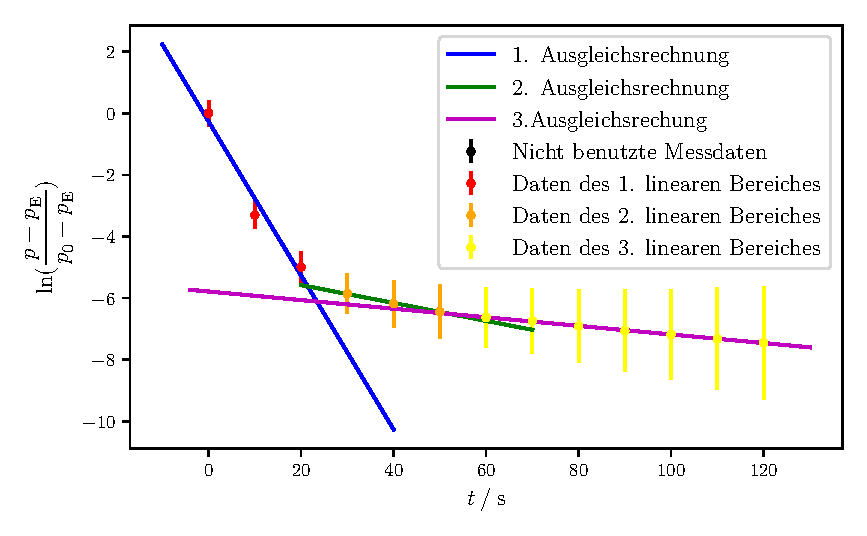
\includegraphics[width=\textwidth]{build/evakuturbo_1_small.pdf}
      \caption{Die Messdaten der ersten Evakuierungsmessung der Turbopumpe aufgetragen in einem Logarithmusausdruck gegen die Zeit. Zusätzlich werden lineare Ausgleichsrechungen in linear wirkende Bereiche gelegt.}
      \label{fig:evaku_turbo_1}
    \end{figure}

    \begin{figure}[h]
      \begin{subfigure}{0.48\textwidth}
        \centering
        \includegraphics[width=\textwidth]{build/evakuturbo_2.pdf}
        \caption{Messung 2}
        \label{fig:turbo_eva_2}
      \end{subfigure}
      \hfill
      \begin{subfigure}{0.48\textwidth}
        \centering
        \includegraphics[width=\textwidth]{build/evakuturbo_3.pdf}
        \caption{Messung 3}
        \label{fig:turbo_eva_3}
      \end{subfigure}
      \caption{Die Messdaten der Evakuierungsmessungen der Turbomolekularpumpe aufgetragen in einem Logarithmusausdruck gegen die Zeit. 
      Zusätzlich werden lineare Ausgleichsrechungen in linear wirkende Bereiche gelegt.}
      \label{fig:turbo_eva_2_3}
    \end{figure}

    % \begin{figure}
      % \centering
      % \includegraphics[width=\textwidth]{build/evakuturbo_2.pdf}
      % \caption{Die Messdaten der zweiten Evakuierungsmessung aufgetragen in einem Logarithmusausdruck gegen die Zeit. Zusätzlich werden lineare Ausgleichsrechungen in linear wirkende Bereiche gelegt.}
      % \label{fig:evaku_turbo_2}
    % \end{figure}

    % \begin{figure}
      % \centering
      % \includegraphics[width=\textwidth]{build/evakuturbo_3.pdf}
      % \caption{Die Messdaten der dritten Evakuierungsmessung aufgetragen in einem Logarithmusausdruck gegen die Zeit. Zusätzlich werden lineare Ausgleichsrechungen in linear wirkende Bereiche gelegt.}
      % \label{fig:evaku_turbo_3}
    % \end{figure}

    \begin{table}[h]
      \centering
      \caption{Die Fitparameter und die daraus errechneten Saugvermögen für die einzelnen Bereiche der Messung.}
      \label{tab:fitpara_turbo_alt}
      \sisetup{table-format=1.4}
      \begin{tabular}{c S[table-format=2.4] @{${}\pm{}$} S S[table-format=2.4] @{${}\pm{}$} S S[table-format=2.4] @{${}\pm{}$} S}
        \toprule
        {Bereiche:} & \multicolumn{2}{c}{$\SI{30}{\nano\bar} \leq p \leq \SI{5000}{\nano\bar}$} & \multicolumn{2}{c}{$\SI{29.9}{\nano\bar} \leq p \leq \SI{17.5}{\nano\bar}$} & \multicolumn{2}{c}{$\SI{17.4}{\nano\bar} \leq p \leq \SI{13.5}{\nano\bar}$}\\
        \midrule
        Messung 1 \\ 
        \cmidrule(lr){1-1}
        $m \mathbin{/} \left(\si{1\per\second}\right)$ & -0.2499 & 0.0465 & -0.0290 & 0.0022 & -0.0139 & 0.0002 \\
        $n$                                            & -0.2687 & 0.6009 & -4.9961 & 0.0889 & -5.7855 & 0.0227 \\
        $S \mathbin{/} \left(\si{L\per\second}\right)$ &  8.2459 & 1.7434 &  0.9583 & 0.1198 &  0.4601 & 0.0467 \\
        \midrule
        Messung 2 \\ 
        \cmidrule(lr){1-1}
        $m \mathbin{/} \left(\si{1\per\second}\right)$ & -0.2660 & 0.0432 & -0.0268 & 0.0013 & -0.0137 & 0.0007 \\
        $n$                                            & -0.2494 & 0.5577 & -5.3131 & 0.0545 & -5.9593 & 0.0641 \\
        $S \mathbin{/} \left(\si{L\per\second}\right)$ &  8.7787 & 1.6742 &  0.8830 & 0.0987 &  0.4537 & 0.0508 \\
        \midrule
        Messung 3 \\ 
        \cmidrule(lr){1-1}
        $m \mathbin{/} \left(\si{1\per\second}\right)$ & -0.2533 & 0.0421 & -0.0265 & 0.0026 & -0.0141 & 0.0007 \\
        $n$                                            & -0.2432 & 0.5439 & -5.2174 & 0.1049 & -5.8293 & 0.0609 \\
        $S \mathbin{/} \left(\si{L\per\second}\right)$ &  8.3573 & 1.6221 &  0.8742 & 0.1218 &  0.4662 & 0.0515 \\      
        \bottomrule
      \end{tabular}
    \end{table}

    \noindent Aus der Steigung der Ausgleichsgeraden kann das Saugvermögen berechnet werden, es gilt der Zusammenhang
    \begin{equation*}
      S = - m \cdot V\, .
    \end{equation*}
    Dies folgt aus der Gleichung \eqref{eqn:saug_eva_theo}. Die entsprechenden Saugvermögen sind auch in der \autoref{tab:fitpara_turbo_alt} aufgelistet. 
    Die Fehler der Werte werden mit der Gleichung \eqref{eqn:err_saug_eva} berechnet.\\ 
    Abschließend werden noch die Mittelwerte berechnet, die wie folgt lauten:
    \begin{align*}
      \SI{30}{\nano\bar} \leq &p \leq \SI{5000}{\nano\bar} & S &= \SI{8.4606 \pm 0.1325}{L\per\second} \\
      \SI{29.9}{\nano\bar} \leq &p \leq \SI{17.5}{\nano\bar}& S &= \SI{0.9052 \pm 0.0218}{L\per\second} \\
      \SI{17.4}{\nano\bar} \leq &p \leq \SI{13.5}{\nano\bar} & S &= \SI{0.4560 \pm 0.0029}{L\per\second}
    \end{align*}
    Hier berechnet sich der Fehler nach Gaußscher Fehlerfortpflanzung nach Gleichung \eqref{eqn:err_anderer_fehler}.

\subsection{Drehschieberpumpe}

    \noindent Nun werden die gleichen Auswertungsschritte bei den Messwerten der Drehschieberpumpe angewendet. Das Volumen des Rezipienten beträgt nun $V = \SI{34 \pm 3.4}{L}$, da die 
    Drehschieberpumpe hinter die dann ausgeschaltete Turbomolekularpumpe geschalten, die Schläuche und die Pumpe, welche nun zusätzlich evakuierten werden müssen, haben also ein Volumen von $V_\text{Zusatz} = \SI{1.0}{L}$. 

    \subsubsection{Leckratenmessung}

    \noindent Analog zum Vorgehen bei der Turbomolekularpumpe wird ein Gleichgewichtsdruck eingestellt. Hier werden die
    Gleichgewichtsdrücke $p_\text{G} = \SI{0.5}{\milli\bar}, \, \SI{10}{\milli\bar}, \, \SI{50}{\milli\bar}, \, \SI{100}{\milli\bar}$ benutzt. Für jeden Gleichgewichtsdruck werden 
    drei Messungen durchgeführt. Der Messzeitraum beträgt $\SI{200}{\second}$, es werden in Schritten von $\increment t = \SI{10}{\second}$ Daten aufgenommen. Über die drei aufgenommenen
    Messungen des Drucks wird das arithmetische Mittel genommen. 
    Die Daten befinden sich für den Gleichgewichtsdruck $p_\text{G} = \SI{0.5}{\milli\bar}$ in der \autoref{tab:dreh_leck_05}, und für $p_\text{G} = \SI{10}{\milli\bar}$ in der 
    \autoref{tab:dreh_leck_10}. Für den Gleichgewichtsdruck $p_\text{G} = \SI{50}{\milli\bar}$ sind die Messdaten in der \autoref{tab:dreh_leck_50} und für $p_\text{G} = \SI{100}{\milli\bar}$
    in der \autoref{tab:dreh_leck_100}.

    \noindent Die gemittelten Drücke werden gegen die Zeit aufgetragen. Dies ist in den Abbildungen in der \autoref{fig:dreh_leck} zu sehen. Dazu sind in lineare Ausgleichsrechnungen 
    mit python \cite{scipy} durchgeführt worden. Die Fitparameter ergeben sich zu:
    \begin{align*}
      \text{Für} \quad  p_\text{G} &= \SI{0.5}{\milli\bar} & \text{Für} \quad  p_\text{G} &= \SI{10}{\milli\bar}\\
      m &= \SI{1.8965(5)e-3}{\milli\bar\per\second} & m &= \SI{0.2313 \pm 0.0018}{\milli\bar\per\second} \\
      n &= \SI{0.4949 \pm 0.0006}{\milli\bar} & n &= \SI{10.1192 \pm 0.2055}{\milli\bar} \\
      \\
      \text{Für} \quad  p_\text{G} &= \SI{50}{\milli\bar} & \text{Für} \quad  p_\text{G} &= \SI{100}{\milli\bar}\\
      m &= \SI{4.7505 \pm 0.2513}{\milli\bar\per\second} & m &= \SI{4.9360 \pm 0.5869}{\milli\bar\per\second} \\
      n &= \SI{-64.3325 \pm 29.3767}{\milli\bar} & n &= \SI{247.5253 \pm 68.6133}{\milli\bar} 
    \end{align*}
    Es werden keine Datenpunkte exkludiert. \\
    Aus dem Steigungen der linearen Ausgleichsrechnung werden die Saugvermögen berechnet durch Vergleich mit Gleichung \eqref{eq:saug_leck_theorie}, wobei sich die Messunsicherheit nach Gleichung \eqref{eqn:err_saug_leck} berechnet:
    \begin{align*}
      \text{für} \quad p_\text{G} &= \SI{0.5}{\milli\bar} & \text{für} \quad p_\text{G} &= \SI{10}{\milli\bar} \\
      S &= \SI{0.1290 \pm 0.0408}{L\per\second}  & S &= \SI{0.7865 \pm 0.2488}{L\per\second}  \\
      \\
      \text{für} \quad p_\text{G} &= \SI{50}{\milli\bar} & \text{für} \quad p_\text{G} &= \SI{100}{\milli\bar} \\
      S &= \SI{3.2303 \pm 1.0357}{L\per\second}  & S &= \SI{1.6782 \pm 0.5670}{L\per\second}  
    \end{align*}

    \begin{figure}[h]
      \begin{subfigure}{0.48\textwidth}
        \centering
        \includegraphics[width=\textwidth]{build/leck_dreh_05mbar.pdf}
        \caption{Gleichgewichtsdruck $p_\text{G} = \SI{0.5}{\milli\bar}$.}
        \label{fig:dreh_leck_05}
      \end{subfigure}
      \hfill
      \begin{subfigure}{0.48\textwidth}
        \centering
        \includegraphics[width=\textwidth]{build/leck_dreh_10mbar.pdf}
        \caption{Gleichgewichtsdruck $p_\text{G} = \SI{10}{\milli\bar}$.}
        \label{fig:dreh_leck_10}
      \end{subfigure}
      \hfill
      \begin{subfigure}{0.48\textwidth}
        \centering
        \includegraphics[width=\textwidth]{build/leck_dreh_50mbar.pdf}
        \caption{Gleichgewichtsdruck $p_\text{G} = \SI{50}{\milli\bar}$.}
        \label{fig:dreh_leck_50}
      \end{subfigure}
      \hfill
      \begin{subfigure}{0.48\textwidth}
        \centering
        \includegraphics[width=\textwidth]{build/leck_dreh_100mbar.pdf}
        \caption{}Gleichgewichtsdruck $p_\text{G} = \SI{100}{\milli\bar}$.
        \label{fig:dreh_leck_100}
      \end{subfigure}
      \caption{Die gemittelten Drücke der Messungen zu den verschiedenen Gleichgewichtsdrücken mit der jeweiligen linearen Ausgleichsrechnung.}
      \label{fig:dreh_leck}
    \end{figure}

  \subsubsection{Evakuierungskurve}

    \noindent Die Drehschieberpumpe hat einen Enddruck von $p_\text{E} = \SI{3.85(115)e-3}{\milli\bar}$. Der Rezipient wird für die Aufnahme der Evakuierungskurve mit der Drehschieberpumpe 
    bis zu einem Druck von $p_0 = \SI{1000}{\milli\bar}$ belüftet. Dann wird die Luftzufuhr abgeschiebert und der Druck in Abhängigkeit der Zeit in 
    Schritten von $\increment t = \SI{10}{\second}$ aufgenommen bist $t = \SI{600}{\second}$ erreicht. Die aufgenommenen Messdaten sind in den Tabelle \ref{tab:dreh_eva} und \ref{tab:dreh_eva2} zu finden. 
    Dort sind außerdem die Ergbnisse der Rechnung 
    \begin{equation*}
      \ln(F) = \ln \left( \frac{p(t) - p_\text{E}}{p_0 - p_\text{E}}\right)
    \end{equation*}
    eingetragen, da diese für jeden Messung einzeln in ein $t - \ln(F)$ Diagramm eingetragen werden. Die Fehler dieses Ausdruckes werden mit der Gleichung \eqref{eqn:err_ln} berechnet.  

    \begin{figure}[h]
      \begin{subfigure}{0.48\textwidth}
        \centering
        \includegraphics[width=\textwidth]{build/evakudreh_1.pdf}
        \caption{Messung 1}
        \label{fig:dreh_eva_1}
      \end{subfigure}
      \hfill
      \begin{subfigure}{0.48\textwidth}
        \centering
        \includegraphics[width=\textwidth]{build/evakudreh_2.pdf}
        \caption{Messung 2}
        \label{fig:dreh_eva_2}
      \end{subfigure}
      \caption{Die Messdaten der Evakuierungsmessungen der Drehschieberpumpe aufgetragen in einem Logarithmusausdruck gegen die Zeit. 
      Zusätzlich werden lineare Ausgleichsrechungen in linear wirkende Bereiche gelegt.}
      \label{fig:dreh_eva_1_2}
    \end{figure}

    % \begin{figure}[h]
      % \centering
      % \includegraphics[width=\textwidth]{build/evakudreh_1.pdf}
      % \caption{Die Messdaten der ersten Evakuierungsmessung der Drehschieberpumpe aufgetragen in einem Logarithmusausdruck gegen die Zeit. Zusätzlich werden lineare Ausgleichsrechungen in linear wirkende Bereiche gelegt.}
      % \label{fig:evaku_dreh_1}
    % \end{figure}

    % \begin{figure}[h]
      % \centering
      % \includegraphics[width=\textwidth]{build/evakudreh_2.pdf}
      % \caption{Die Messdaten der zweiten Evakuierungsmessung der Drehschieberpumpe aufgetragen in einem Logarithmusausdruck gegen die Zeit. Zusätzlich werden lineare Ausgleichsrechungen in linear wirkende Bereiche gelegt.}
      % \label{fig:evaku_dreh_2}
    % \end{figure}

    \begin{figure}[h]
      \centering
      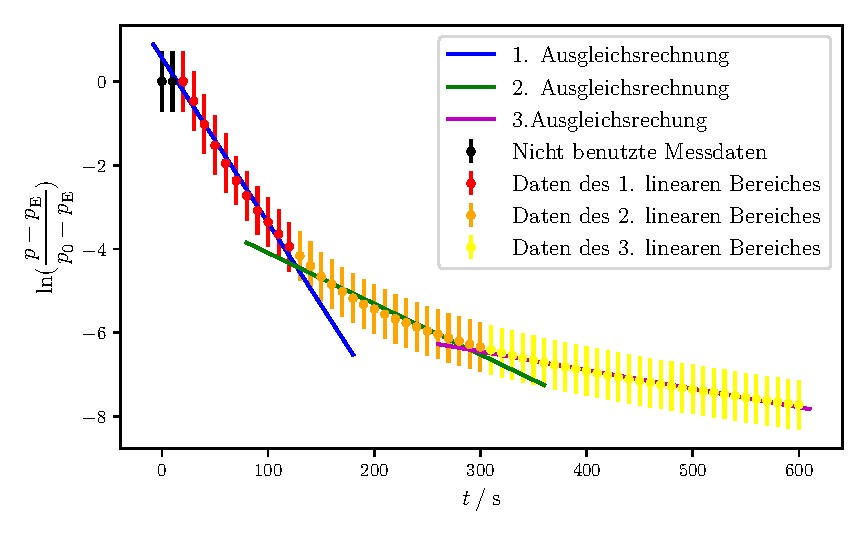
\includegraphics[width=\textwidth]{build/evakudreh_3_small.pdf}
      \caption{Die Messdaten der dritten Evakuierungsmessung der Drehschieberpumpe aufgetragen in einem Logarithmusausdruck gegen die Zeit. Zusätzlich werden lineare Ausgleichsrechungen in linear wirkende Bereiche gelegt.}
      \label{fig:evaku_dreh_3}
    \end{figure}

    \noindent Die Abbildungen werden auf lineares Verhalten untersucht, wobei jeweils drei verschiedene Bereiche mit linearem Verhalten identifiziert werden. 
    Dies ist für die Messreihe 1 in der \autoref{fig:dreh_eva_1}, für die Messreihe 2 in der \autoref{fig:dreh_eva_2} und für die dritte Messreihe in der 
    \autoref{fig:evaku_dreh_3} zu sehen. Bei der dritten Messreihe werden die ersten beiden Datenpunkte exkludiert, da diese so gut wie gleich dem dritten Punkt sind und sich 
    daher vermuten lässt, dass die Zeitnahme begonnen hat, bevor der Rezipient komplett abgedichtet war.\\ 
    Die Parameterdaten der linearen Ausgleichsrechnungen sind in der Tabelle \autoref{tab:fitpara_dreh_alt} aufgelistet für die verschiedenen Druckbereichen. Das Saugvermögen berechnet sich 
    aus der Steigung $m$ durch 
    \begin{equation*}
      S = m \cdot V\, ,
    \end{equation*}
    welches sich durch Vergleich mit Gleichung \eqref{eqn:saug_eva_theo} ergibt.
    Die Werte für das Saugvermögen sind auch in der \autoref{tab:fitpara_dreh_alt} aufgelistet, der Fehler berechnet sich nach der Formel \eqref{eqn:err_saug_leck}. 

    \begin{table}[h]
      \centering
      \caption{Die Fitparameter und die daraus errechneten Saugvermögen für die einzelnen Bereiche der Messungen von der Evakuierungskurve der Drehschieberpumpe.}
      \label{tab:fitpara_dreh_alt}
      \sisetup{table-format=1.4}
      \begin{tabular}{c | S[table-format=2.4] @{${}\pm{}$} S  S[table-format=2.4] @{${}\pm{}$} S  S[table-format=2.4] @{${}\pm{}$} S}
        \toprule
        {Bereiche:} & \multicolumn{2}{c}{$\SI{10}{\milli\bar} \leq p \leq \SI{1000}{\milli\bar}$} & \multicolumn{2}{c}{$\SI{1.5}{\milli\bar} \leq p \leq \SI{10}{\milli\bar}$} & \multicolumn{2}{c}{$\SI{0.4}{\milli\bar} \leq p \leq \SI{1.5}{\milli\bar}$}\\
        \midrule
        Messung 1 \\ 
        \cmidrule(lr){1-1}
        $m \mathbin{/} \left(\si{1\per\second}\right)$ & -0.0371 & 0.0014 & -0.0106 & 0.0004 & -0.0043 & 0.0001 \\
        $n$                                            & -0.1380 & 0.0956 & -3.3976 & 0.0929 & -5.2577 & 0.0282 \\
        $S \mathbin{/} \left(\si{L\per\second}\right)$ &  1.2628 & 0.1344 &  0.3612 & 0.0388 &  0.1458 & 0.0147 \\
        \midrule
        Messung 2 \\ 
        \cmidrule(lr){1-1}
        $m \mathbin{/} \left(\si{1\per\second}\right)$ & -0.0367 & 0.0013 & -0.0108 & 0.0004 & -0.0043 & 0.0001 \\
        $n$                                            & -0.1281 & 0.0901 & -3.3426 & 0.0992 & -5.2454 & 0.0289 \\
        $S \mathbin{/} \left(\si{L\per\second}\right)$ &  1.2475 & 0.1321 &  0.3670 & 0.0397 &  0.1462 & 0.0148 \\
        \midrule
        Messung 3 \\ 
        \cmidrule(lr){1-1}
        $m \mathbin{/} \left(\si{1\per\second}\right)$ & -0.0394 & 0.0015 & -0.0121 & 0.0006 & -0.0044 & 0.0001 \\
        $n$                                            &  0.5661 & 0.1173 & -2.8796 & 0.1314 & -5.1153 & 0.0320 \\
        $S \mathbin{/} \left(\si{L\per\second}\right)$ &  1.3389 & 0.1436 &  0.4125 & 0.0459 &  0.1508 & 0.0153 \\      
        \bottomrule
      \end{tabular}
    \end{table}

    \noindent Es werden über die einzelnen Bereiche der Mittelwert der pro Messung berechneten Saugvermögen berechnet. Diese Werte ergeben sich zu:
    \begin{align*}
      \SI{10}{\nano\bar} \leq &p \leq \SI{1000}{\nano\bar} & S &= \SI{1.2830 \pm 0.0789}{L\per\second} \\
      \SI{1.5}{\nano\bar} \leq &p \leq \SI{10}{\nano\bar}& S &= \SI{0.3802 \pm 0.0240}{L\per\second} \\
      \SI{0.4}{\nano\bar} \leq &p \leq \SI{1.5}{\nano\bar} & S &= \SI{0.1476 \pm 0.0086}{L\per\second}
    \end{align*}
    Hier wird der Fehler aus der Fehlerfortpflanzung nach Gauß nach Gleichung \eqref{eqn:err_anderer_fehler} berechnet. 